\chapter*{Conclusion}\label{chapter:concl}
\addcontentsline{toc}{chapter}{Conclusion} \mtcaddchapter
\markboth{Conclusion}{Conclusion}
 
\noindent Au cours du travail de thèse ici présenté, nous nous sommes intéressés principalement aux interactions entre atomes de Rydberg.
Les atomes de Rydberg alcalins, décrits par la théorie du défaut quantique, présentent une très grande taille, un très long temps de vie, et de très grands dipôles électriques de transition.
Grâce à ces grands dipôles, les atomes de Rydberg interagissent entre eux beaucoup plus fortement que les atomes dans l'état fondamental, et à des distances bien plus grandes.
Dans les cas qui nous intéressent, cette interaction prend une forme de van der Waals en $1/r^6$.

Les expériences que nous avons décrites dans le présent manuscrit ont été réalisées au sein d'un dispositif expérimental hybride, adapté à la fois aux techniques du piégeage et du refroidissement d'atomes dans leur état fondamental et à l'excitation, la détection et la  manipulation d'atomes de Rydberg.
Grâce à ce dispositif, nous pouvons capturer des atomes de rubidium $87$ devant une puce à atomes, les piéger dans des pièges magnéto-optiques ou magnétiques, et les refroidir, d'abord par laser puis par évaporation, jusqu'à %proximité de 
la condensation de Bose-Einstein.
\`A partir des nuages d'atomes ultra-froids ainsi créés, nous excitons des atomes de Rydberg par une transition laser à deux photons, naviguons entre niveaux de Rydberg voisins grâce à des sources externes de champ microonde, puis détectons les atomes de Rydberg par ionisation sélective.

Au sein de ce dispositif, nous avons pu mettre en évidence les effets de l'interaction dipolaire sur l'excitation et le mouvement d'un ensemble dense d'atomes de Rydberg.
Ces effets sont le blocage dipolaire, qui interdit l'excitation de deux atomes de Rydberg séparés d'une distance trop petite, l'excitation facilitée au cours de laquelle un désaccord positif du laser d'excitation crée une région où l'excitation de nouveaux atomes de Rydberg devient résonante, et l'expansion du nuage de Rydberg sous l'effet répulsif des interactions.
Le blocage dipolaire et l'excitation facilitée sont mis en évidence par la spectroscopie laser de la transition depuis le niveau fondamental $\mathrm{5S}$ vers le niveau de Rydberg $\mathrm{60S}$.
Le mouvement relatif d'un ensemble d'atomes de Rydberg est mis en évidence par la spectroscopie microonde de la transition $\mathrm{60S \rightarrow 57S}$ au cours de l'expansion.
Un modèle numérique Monte-Carlo permet de simuler l'excitation et le mouvement d'un gaz dense d'atomes de Rydberg, et de reproduire les données expérimentales de façon relativement satisfaisante.

Les interactions dipolaires font des atomes de Rydberg une \og brique élémentaire \fg{} prometteuse pour la réalisation d'un simulateur quantique.
Nous avons ainsi présenté une proposition expérimentale détaillée de simulateur quantique, constitué d'atomes de Rydberg circulaires en interaction, piégés par laser et dont la durée de vie est préservée par inhibition de la désexciation par émission spontanée.
Une méthode analogue au refroidissement évaporatif permet en outre de préparer de façon déterministe une chaîne régulière et sans défaut d'une quarantaine d'atomes de Rydberg circulaires.
Ce simulateur présente de nombreux avantages : il permettrait de réaliser un hamiltonien $\mathrm{XXZ}$ entièrement modulable, simulant une chaîne d'une quarantaine de spins $1/2$ en interaction pendant des durées de l'ordre de $\SIrange{e4}{e5}{}$ temps caractéristiques d'échange.

En vue de réaliser ce simulateur il nous a fallu nous intéresser aux atomes de Rydberg circulaires, c'est-à-dire dont le moment cinétique et sa projection sont maximales.
Une étape particulière est nécessaire à l'excitation d'atomes de Rydberg circulaires : le passage adiabatique radio-fréquence.
Nous avons adapté le dispositif expérimental afin de pouvoir effectuer ce passage adiabatique, en installant un jeu de quatre électrodes supplémentaires capable de générer des champs électriques radio-fréquence polarisés dans le plan parallèle à la puce à atomes.
Grâce à ces électrodes, nous avons excités des atomes de Rydberg dans le niveau circulaire $\mathrm{50C}$ depuis le niveau fondamental, en passant par l'excitation laser du niveau $\mathrm{50D_{5/2}}$ puis par le transfert microonde vers le niveau $\mathrm{50F}$, à partir duquel commence le passage adiabatique radio-fréquence.
L'analyse des signaux d'ionisation, puis la spectroscopie microonde de la transition $\mathrm{50C \rightarrow 51C}$ permettent de caractériser les atomes de Rydberg circulaires que nous excitons.

\bigskip
%Les perspectives à court terme 
Notre proposition de simulateur quantique représente un projet à long terme ambitieux et les efforts expérimentaux pour y parvenir seront importants.
La première étape de ce chemin sera la démonstration du piégeage des atomes de Rydberg circulaires dans un faisceau laser.

Notre première idée consistait à laisser tomber les atomes par gravité, jusqu'à ce qu'ils sortent de la région où ils peuvent être détectés.
La présence du laser de piégeage aurait alors pour conséquence d'empêcher la chute libre des atomes de Rydberg circulaires.
Malheureusement, les premières estimations expérimentales, sans inhibition de l'émission spontanée, montrent une durée de vie du niveau circulaire $\mathrm{50C}$ trop courte pour observer la chute libre.
En effet, avec une durée de vie de l'ordre de $\SI{2}{\ms}$, les atomes ne tombent que d'environ $\SI{20}{\um}$ avant d'être désexcités.

Nous attribuons la réduction de durée de vie actuelle à la présence de rayonnement du corps noir, qui passe à travers les hublots d'accès optique du cryostat et stimule des transitions de désexcitation.
Des efforts sont déjà mis en \oe uvre afin de réduire le nombre de ces photons, en plaçant des matériaux absorbants pour le rayonnement microonde à l'intérieur de l'enceinte à $\SI{4.2}{\K}$ du cryostat.

Une autre piste que nous souhaitons explorer consiste à déplacer les atomes de Rybderg circulaires grâce au faisceau de piégeage.
Il s'agirait, une fois les atomes excités, d'allumer le faisceau de piégeage, de le déplacer vers le bas puis de le ramener à sa position initiale, le tout grâce à un modulateur acousto-optique.
La profondeur du potentiel créé par le laser est suffisante pour communiquer aux atomes des accélérations de l'ordre de $\SI{450}{}\times g$ sans risquer de les faire sortir du piège.
Une telle accélération permet un déplacement des atomes de l'ordre de $\SI{2}{\mm}$ en $\SI{1}{\ms}$.
Les atomes de Rydberg devraient alors suivre le faisceau de piégeage et être toujours détectables après leur aller-retour.
Une situation légèrement différente servirait alors de référence : le laser de piégeage est allumé puis déplacé vers le bas, et éteint de façon à communiquer aux atomes la plus forte accélération possible, ce qui les propulsera en dehors de la zone de détection.

Le faisceau creux de piégeage transverse le long de l'axe $Ox$ a déjà été préparé, grâce à une lame de phase qui permet de créer un profil de Laguerre-Gauss d'ordre $1$ au niveau du col du faisceau focalisé.
Ce faisceau creux est prêt à être caractérisé et à être utilisé dans nos premières expériences de démonstration du piégeage laser des atomes de Rydberg circulaires.
Dans tous les cas, il sera nécessaire d'estimer et d'améliorer au maximum la durée de vie des niveaux circulaires au sein du dispositif actuel, même si celui-ci ne permet pas encore l'inhibition de l'émission spontanée.


\bigskip
%Les perspectives à long terme
La progression ultérieure vers la réalisation du simulateur quantique nécessitera une refonte importante du dispositif expérimental.
En premier lieu, le cryostat devra être adapté à l'utilisation de l'hélium $3$, permettant d'atteindre des températures de l'ordre de $\SI{0.4}{\K}$.
Il faudra ensuite modifier la disposition des éléments centraux du dispositif, et y intercaler un condensateur d'inhibition de l'émission spontanée.
La puce à atomes permettant le piégeage et le refroidissement des atomes dans l'état fondamental se trouvera d'un côté de ce condensateur, et le dispositif de détection par ionisation des atomes de Rybderg de l'autre côté.
La figure \eqref{fig:simul_setup} présente un schéma de principe de ce dispositif modifié.
%
\begin{figure}[t]
\centering
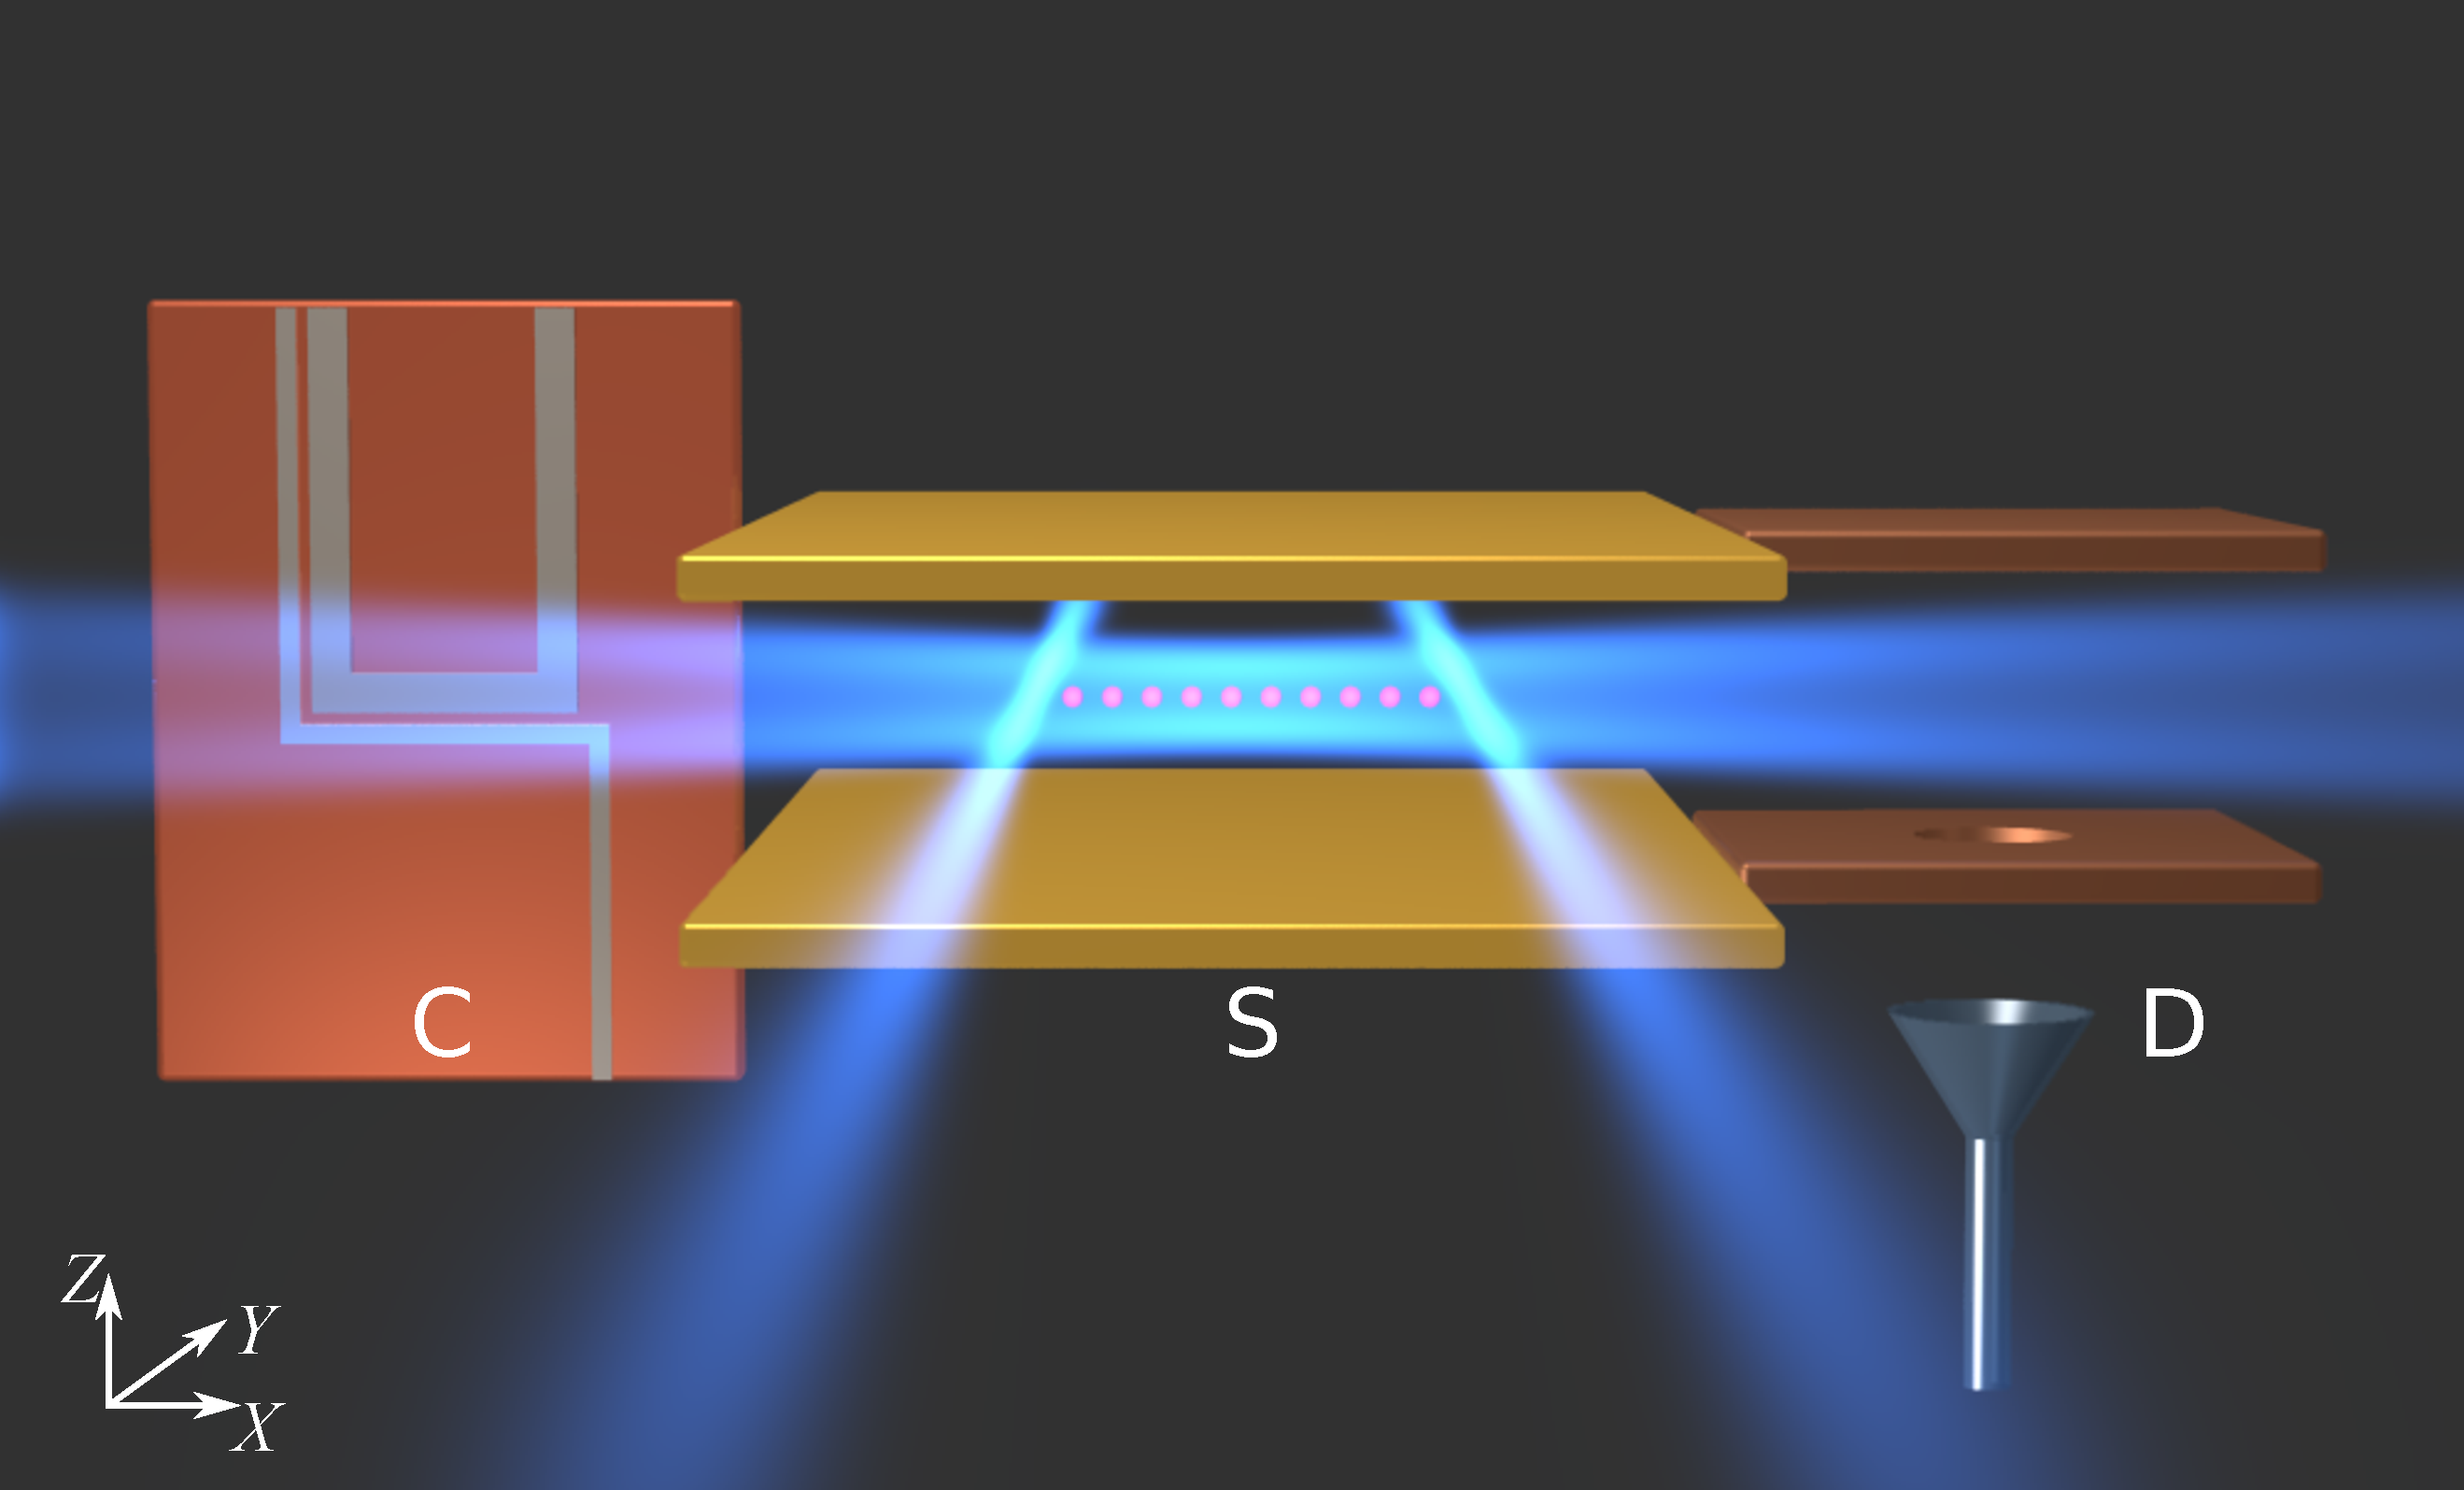
\includegraphics[width=0.6\linewidth]{figures/compscheme}
\caption[Schéma de principe du dispositif expérimental adapté au simulateur quantique]{
Schéma de principe du dispositif expérimental adapté au simulateur quantique.
Les atomes dans l'état fondamental sont piégés et refroidis devant la puce $(C)$ puis transportés dans le condensateur de science $(S)$.
Dans ce condensateur, la chaîne d'atomes de Rydberg et préparée et la simulation a lieu.
Les atomes de Rydberg sont ensuite envoyés un par un dans la zone de détection $(D)$ où ils sont ionisés.
}
\label{fig:simul_setup}
\end{figure}
%

Au sein de ce futur dispositif, les atomes dans l'état fondamental seront piégés et refroidis devant une puce à atomes.
Ils sont ensuite piégés dans un piège dipolaire rouge et transportés à l'intérieur du condensateur, où ils sont excités vers un niveau de Rydberg de bas moment cinétique.
Enfin, les atomes de Rydberg sont \og circularisés \fg{} à l'intérieur même du condensateur, grâce à quatre électrodes, situées chacune à un coin de l'une des deux plaques constituant le condensateur, générant un champ radio-fréquence évanescent polarisé $\sigma^+$.
Une fois excités, les atomes de Rydberg circulaires seront piégés le long de l'axe $Ox$ dans un faisceau creux, puis préparés de façon déterministe en une chaîne régulière de quarante atomes par la méthode présentée au chapitre \ref{chapter:circsim}, et enfin piégés longitudinalement par un réseau optique.
\`A la fin de la simulation, ils seront éjectés un par un vers la zone de détection où ils seront ionisés.

Au-delà de l'adaptation du dispositif interne au cryostat, un travail important d'optique sera nécessaire, afin de créer l'ensemble des faisceaux de piégeage à $\SI{1064}{\nano\meter}$, ainsi que le faisceau de piégeage dipolaire des atomes dans l'état fondamental, et les faisceaux \og bouchons \fg{} servant à la préparation de la chaîne.
%Parmi ceux-ci, le faisceau creux de piégeage transverse le long de l'axe $Ox$ a déjà été préparé, grâce à une lame de phase qui permet de créer un profil de Laguerre-Gauss d'ordre $1$ au niveau du col du faisceau focalisé.
%Ce faisceau creux est prêt à être caractérisé et à être utilisé dans nos premières expériences de démonstration du piégeage laser des atomes de Rydberg circulaires.

\bigskip
%La physique simulée
Le simulateur quantique que nous proposons permet de s'intéresser à des problèmes passionnants de la physique quantique à $N$ corps.
Nous conclurons le présent manuscrit en en évoquant quelques uns.

La première étape de fonctionnement du simulateur sera sa caractérisation et sa validation (\textit{benchmarking}), en comparant ses résultats à des phases connues, ainsi qu'à des transitions de phases simples.
Le contrôle des paramètres du hamiltonien pouvant être fait très rapidement, il sera ensuite possible de simuler des trempes.
Ces variations brutales des paramètre du hamiltonien induisent des phénomènes hors équilibre particulièrement intéressants.
Il s'agirait tout d'abord de savoir si le système qui subit une trempe peut revenir à une situation d'équilibre, ce qui n'est pas garanti dans le cas d'un système quantique isolé.
Ensuite, si de tels processus d'équilibrage et de thermalisation sont à l'\oe uvre, il s'agira de les caractériser, tout particulièrement dans un régime de temps de relaxation intermédiaire où l'on pourrait suivre la propagation des corrélations au sein du système.

L'introduction de désordre au sein de la chaîne d'atomes de Rydberg circulaires est chose aisée, en ajoutant au réseau laser de piégeage un motif de tavelures (\textit{speckle}).
Les atomes seraient alors déplacés aléatoirement de leur position initiale, créant une chaîne irrégulière.
Cela permettrait l'étude des processus de transport et de localisation d'une ou plusieurs excitation au sein d'une chaîne désordonnée, menant la physique des verres de Bose ou à l'émergence de phases singulet aléatoires.

Enfin, l'on peut imaginer augmenter la dimension du système de spins simulé.
Le premier stade d'une telle extension du simulateur consisterait à accoler deux chaînes régulières d'atomes de Rydberg circulaires, de façon à former ce que l'on pourrait appeler une \og échelle \fg{} de spins.
L'anisotropie des interactions entre atomes de Rydberg circulaires permettrait alors de réaliser un couplage entre atomes des deux chaînes de signe opposé au couplage entre les atomes au sein de chaque chaîne.
La géométrie en échelle réaliserait alors une phase de Haldane pour des particules de spin $1$.
Cette phase de Haldane possède un ordre topologique non trivial et des états de bord de spin $1/2$ (\textit{spin 1/2 edge states}) qui sont d'un grand intérêt.

Une extension à deux ou trois dimensions de la méthode de préparation de chaîne pourrait amener notre proposition de simulateur quantique vers des problèmes ou la compréhension même de l'état fondamental du système n'est pas assurée.
C'est là une perspective enthousiasmante d'investigation expérimentale, dans des domaines où l'étude théorique d'aujourd'hui semble trouver ses limites.


%
%
%1. les phases du hamiltonien xxz. défauts -> Kibble Zurek
%
%2. désordre dans la chaîne -> localisation vs interaction -> verre de Bose (+ singulet aléatoire ??)
%
%3. modulation du hamiltonien -> excitations élémentaires du système, en particulier de basse énergie grâce au très long temps de vie
%
%4. physique de Floquet avec modulation très rapide
%
%5. trempes instantanées -> équilibrage et thermalisation, préthermalisation, lien avec l'intégrabilité, déphasage d'un sous-système, many-body localization
%
%6. couplage spin-mouvement
%
%7. physique de Haldane avec deux chaînes formant une échelle, et perspectives plus générales à 2 et 3 D.